\documentclass[a4paper]{article}
\usepackage{amsmath,amssymb,caption,float,graphicx,minted,xcolor}
\usepackage[utf8]{inputenc}
\usepackage[english]{babel}
\usepackage[backend=bibtex]{biblatex}
\addbibresource{Lab3.bib}
\captionsetup[figure]{labelsep=period}
\definecolor{bg}{rgb}{0.95,0.95,0.95}
\renewcommand\thesection{\arabic{section}}
\usemintedstyle{emacs}
\begin{document}
\begin{center}
    \huge
    \textbf{VE482\\Introduction to Operating Systems\\}
    \Large
    \vspace{15pt}
    \uppercase{\textbf{Lab 3}}\\
    \large
    \vspace{5pt}\today\\
    \vspace{5pt}
    Yihua Liu 518021910998
    \vspace{5pt}
    \rule[-5pt]{.97\linewidth}{0.05em}
\end{center}
\section{Project 1: presentations (part 2)}
\section{Working with source code}
\subsection{The \texttt{rsync} command}
\begin{itemize}
    \item In Minix 3 install the \texttt{rsync} software
    \begin{minted}[frame=single,bgcolor=bg,breaklines,linenos]{bash}
        pkgin install rsync
    \end{minted}
    \item Install \texttt{rsync} on you Linux system
    \texttt{rsync} has already installed on my WSL Ubuntu and Ubuntu VMware virtual machine.
    \item Read \texttt{rsync} manpage
    \begin{minted}[frame=single,bgcolor=bg,breaklines,linenos]{bash}
        man rsync
    \end{minted}
    \item Create an exact copy of the directory \texttt{/usr/src} into the directory \texttt{/usr/src\_orig}
    \begin{minted}[frame=single,bgcolor=bg,breaklines,linenos]{bash}
        cp -r /usr/src/ /usr/src_orig
    \end{minted}
    \item If you have already altered Minix 3 source code for homework 2 undo your changes from \texttt{/usr/src\_orig}
    I have not altered Minix 3 source code for homework 2.
    \item Create an exact copy of the Minix 3 directory \texttt{/usr/src} into your Linux system, using \texttt{rsync} and \texttt{ssh} (note that the \texttt{ssh} server must be activated under Linux)
    \begin{minted}[frame=single,bgcolor=bg,breaklines,linenos]{bash}
        rsync -avz minix:/usr/src /mnt/f/Resources
    \end{minted}
    Here \texttt{minix} is the host that we have added before.\\
    The meanings of the options are \cite{rsync}:
    -a, --archive               archive mode; equals -rlptgoD (no -H,-A,-X)\\
    -v, --verbose               increase verbosity\\
    -z, --compress              compress file data during the transfer
    \begin{figure}[H]
        \centering
        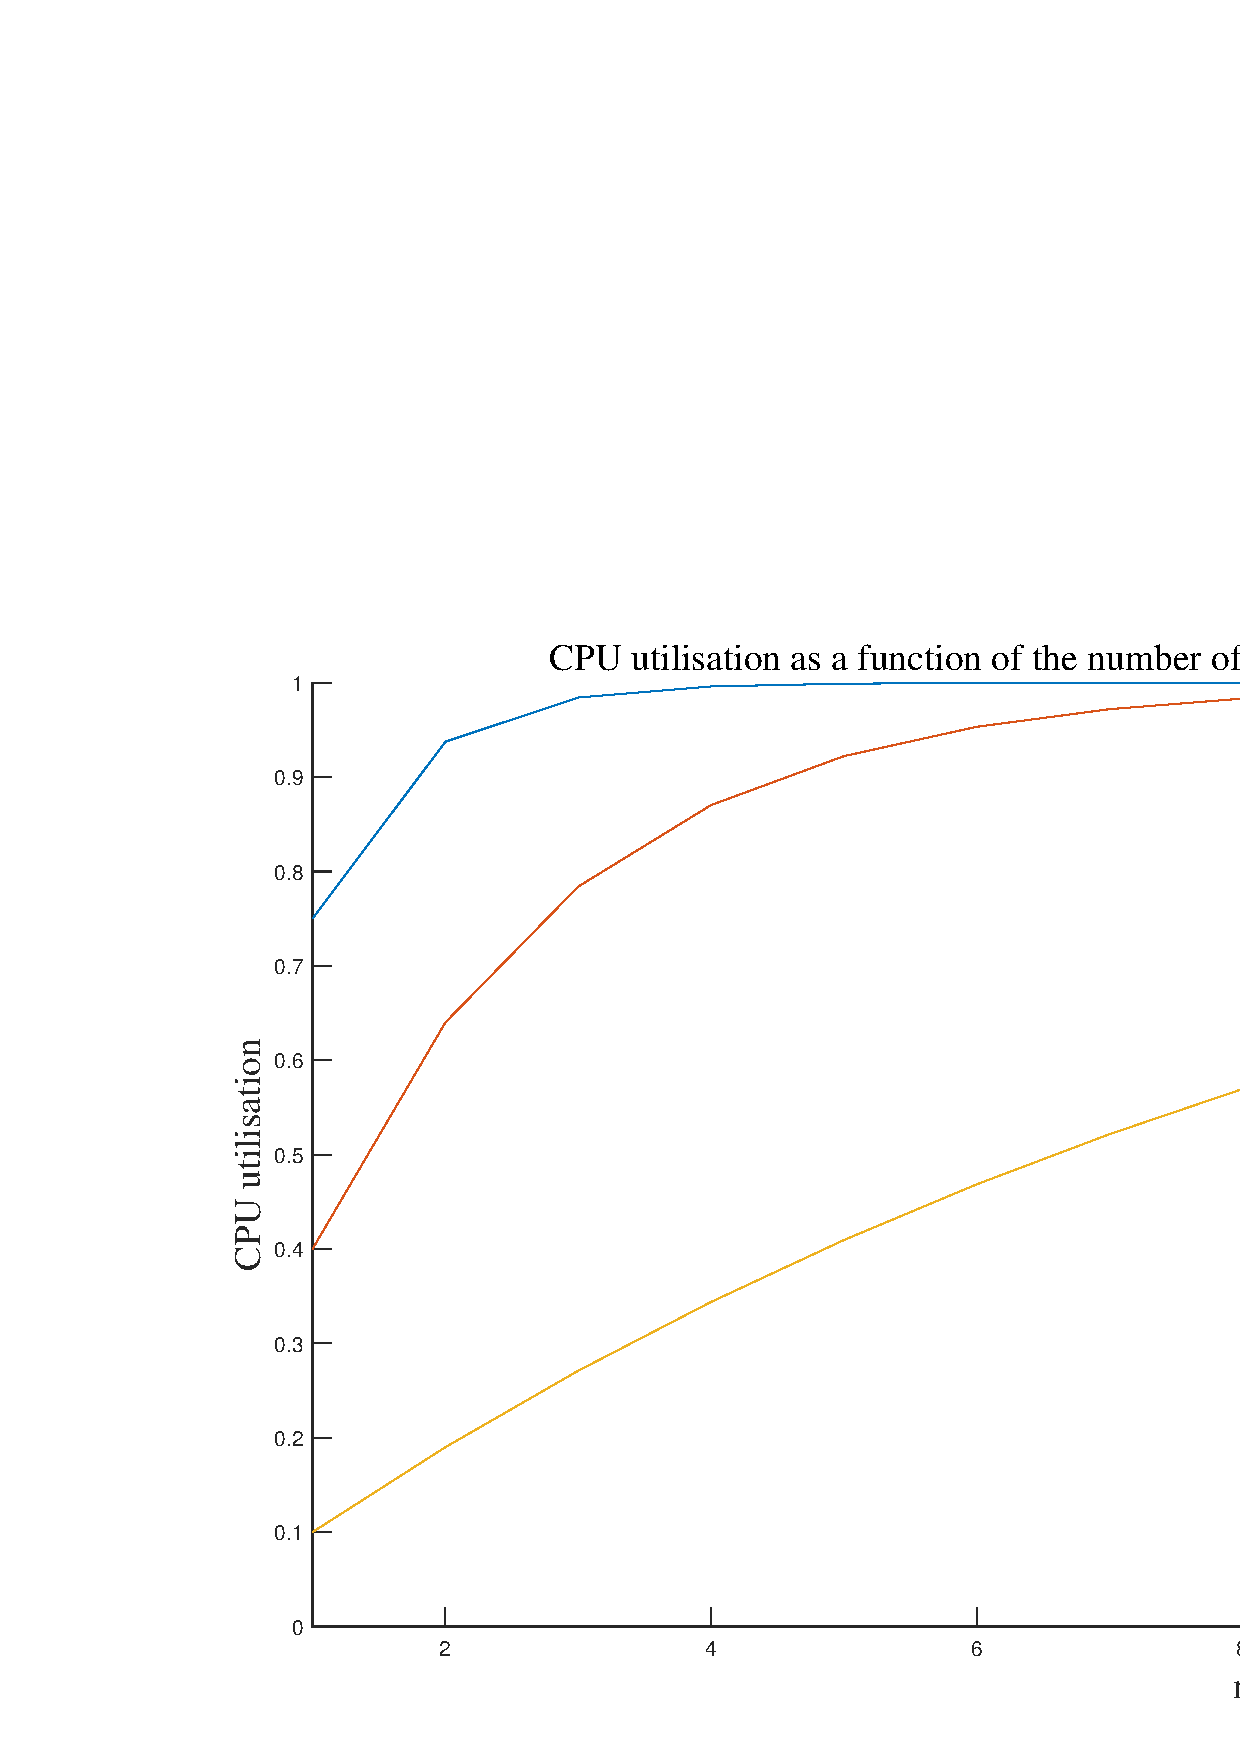
\includegraphics[width=0.8\textwidth]{1.png}
        \caption{Output of \texttt{rsync} command.}
    \end{figure}
    Note: you cannot run \texttt{rsync} under Minix 3 like
    \begin{minted}[frame=single,bgcolor=bg,breaklines,linenos]{bash}
        rsync -a /usr/src ubuntu:~/
    \end{minted}
    \begin{figure}[H]
        \centering
        \includegraphics[width=0.8\textwidth]{2.png}
        \caption{System panicked if \texttt{rsync} under Minix 3.}
    \end{figure}
\end{itemize}
\subsection{The \texttt{diff} and \texttt{patch} commands}
\begin{itemize}
    \item Read the manpages of \texttt{diff} and \texttt{patch}
    \begin{minted}[frame=single,bgcolor=bg,breaklines,linenos]{bash}
        man diff
        man patch
    \end{minted}
    \item Edit a file of your choice in \texttt{/usr/src}, e.g. add a comment to a file
    \begin{minted}[frame=single,bgcolor=bg,breaklines,linenos]{bash}
        vi /usr/src/build.sh  # Add an empty comment in the beginning
    \end{minted}
    \item Using the \texttt{diff} command, create a patch corresponding to the above changes
    \begin{minted}[frame=single,bgcolor=bg,breaklines,linenos]{bash}
        diff /usr/src_orig/build.sh /usr/src/build.sh > build.patch
    \end{minted}
    \item Retrieve your patch on your Linux system
    \begin{minted}[frame=single,bgcolor=bg,breaklines,linenos]{bash}
        rsync -avz minix:~/build.patch ~
    \end{minted}
    \item Apply your patch to the copy of \texttt{/usr/src\_orig} on your Linux system
    \begin{minted}[frame=single,bgcolor=bg,breaklines,linenos]{bash}
        patch -p0 build.sh ~/build.patch
    \end{minted}
    \item Revert the patch
    \begin{minted}[frame=single,bgcolor=bg,breaklines,linenos]{bash}
        patch -R build.sh ~/build.patch
    \end{minted}
\end{itemize}
\begin{figure}[H]
    \centering
    \includegraphics[width=0.8\textwidth]{3.png}
    \caption{Retrieving, applying, and reverting the patch on Linux system.}
\end{figure}
\subsection{Remarks}
\subsection{Basic git usage}
\begin{figure}[H]
    \centering
    \includegraphics[width=0.8\textwidth]{4.png}
\end{figure}
\begin{figure}[H]
    \centering
    \includegraphics[width=0.8\textwidth]{5.png}
\end{figure}
\begin{figure}[H]
    \centering
    \includegraphics[width=0.8\textwidth]{6.png}
\end{figure}
\begin{figure}[H]
    \centering
    \includegraphics[width=0.8\textwidth]{7.png}
\end{figure}
\begin{figure}[H]
    \centering
    \includegraphics[width=0.8\textwidth]{8.png}
\end{figure}
\begin{figure}[H]
    \centering
    \includegraphics[width=0.8\textwidth]{9.png}
\end{figure}
\begin{figure}[H]
    \centering
    \includegraphics[width=0.8\textwidth]{10.png}
\end{figure}
\begin{figure}[H]
    \centering
    \includegraphics[width=0.8\textwidth]{11.png}
\end{figure}
\begin{figure}[H]
    \centering
    \includegraphics[width=0.8\textwidth]{12.png}
\end{figure}
\begin{figure}[H]
    \centering
    \includegraphics[width=0.8\textwidth]{13.png}
\end{figure}
\begin{figure}[H]
    \centering
    \includegraphics[width=0.8\textwidth]{14.png}
\end{figure}
\begin{figure}[H]
    \centering
    \includegraphics[width=0.8\textwidth]{15.png}
\end{figure}
\begin{figure}[H]
    \centering
    \includegraphics[width=0.8\textwidth]{16.png}
\end{figure}
\begin{figure}[H]
    \centering
    \includegraphics[width=0.8\textwidth]{17.png}
\end{figure}
\begin{figure}[H]
    \centering
    \includegraphics[width=0.8\textwidth]{18.png}
\end{figure}
\begin{figure}[H]
    \centering
    \includegraphics[width=0.8\textwidth]{19.png}
\end{figure}
\begin{figure}[H]
    \centering
    \includegraphics[width=0.8\textwidth]{20.png}
\end{figure}
\begin{figure}[H]
    \centering
    \includegraphics[width=0.8\textwidth]{21.png}
\end{figure}
\section{Scripting and regular expressions}
\begin{minted}[frame=single,bgcolor=bg,breaklines,breakanywhere,linenos]{bash}
    curl "https://aqicn.org/?city=Shanghai&widgetscript&size=large" 2>/dev/null | sed -nE 's/.*title=\\"Moderate\\">([[:digit:]]{1,3}).*>([-]?[[:digit:]]{1,5})<\\\/td><\\\/tr><\\.*/AQ: \1 Temp: \2 ºC/p'
\end{minted}
\begin{minted}[frame=single,bgcolor=bg,breaklines,linenos]{bash}
    ifconfig | awk -e '{for (i = 1; i <= NF; ++i) {if ($i=="inet") {printf $(i+1)"\n"}}}'
\end{minted}
\printbibliography
\end{document}